\documentclass{article}
\usepackage{graphicx}
\graphicspath{ {images/} }
\usepackage{float}

% alternative font if you prefer
% \usepackage{times}

% for alternative page numbering use the following package
% and see documentation for commands
\usepackage{fancyheadings}
\usepackage{hyperref}


% other potentially useful packages
\usepackage{amssymb,amsmath}
%\usepackage{url}
%\usepackage{fancyvrb}
%\usepackage[final]{pdfpages}
\setlength{\parindent}{0pt}
\setlength{\parskip}{11pt plus 2pt}

\begin{document}

%%%%%%%%%%%%%%%%%%%%%%%%%%%%%%%%%%%%%%%%%%%%%%%%%%%%%%%%%%%%%%%%%%%
\title{Report: Generative Processes of Static and Dynamic LDA Models}
\author{Arijus Pleska}
\maketitle

%%%%%%%%%%%%%%%%%%%%%%%%%%%%%%%%%%%%%%%%%%%%%%%%%%%%%%%%%%%%%%%%%%%

% - Comparing the static and dynamics models.
% - Questions 
\par During this week I have familiarised with the generative processes of static and dynamic LDA models. In this report I will present the results by plotting the generated documents, address the estimation of the parameters $\alpha$ and $\beta$, and raise questions to be considered for the next meeting.

% Generative process
\par I have managed to generate documents using both static and dynamic variations. The static approach in generating corpus is given in Figure 1, and the dynamic approach is given in Figure 2.

\begin{figure}[H]
  \centering
  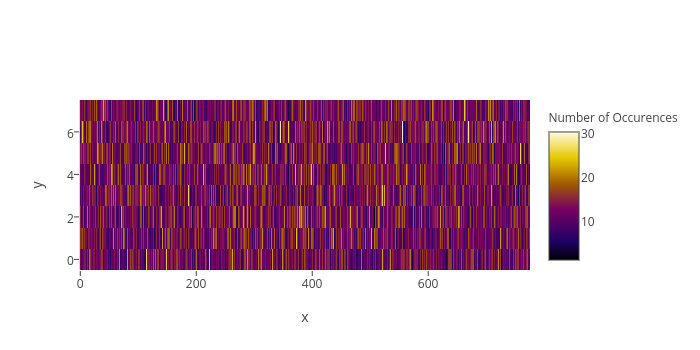
\includegraphics[width=\textwidth]{static}
  \caption{The distribution of a word in a corpus produced by the static generative process.}
  \label{fig:static}
\end{figure}

\begin{figure}[H]
  \centering
  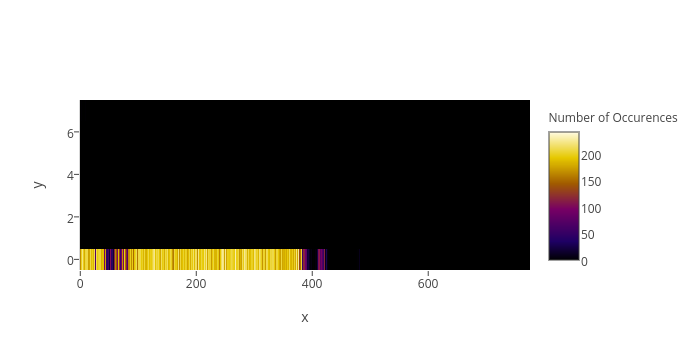
\includegraphics[width=\textwidth]{dynamic}
  \caption{The distribution of a word in a corpus produced by the dynamic generative process.}
  \label{fig:dynamic}
\end{figure}

In Figure 1 we can see that the word is present throughout all the corpus, whereas Figure 2 displays a smoother distribution of the word. That is, the dynamic generative process induces a structure of the word's existence in the corpus. Also, note that both corpus contain the same number of documents and the number of words in a document is drawn from the Poisson distribution on the same mean $\xi = 200$.

The implementation of the generative processes follow directly from the original LDA paper \cite{Blei:2003:LDA:944919.944937} and the paper on dynamic topic models \cite{Blei:2006:DTM:1143844.1143859}. The Python Notebook containing the implementation of the processes can be found by using the following link: \url{https://github.com/perdaug/mlinb/blob/master/notebooks/generating_corpus.ipynb}.

\bibliographystyle{unsrt}
\bibliography{report_generative-process}

\end{document}
